% ============================================================
\chapter{Codes-Barres et Diagrammes de Persistance}
\label{ch:diagrammes}
% ============================================================

L'homologie persistante produit une quantit\'e consid\'erable d'information~: pour chaque dimension, une liste de caract\'eristiques topologiques avec leurs dates de naissance et de mort. Comment visualiser et comparer ces r\'esultats~? Deux repr\'esentations \'equivalentes se sont impos\'ees~: le \emph{code-barres}, o\`u chaque caract\'eristique est une barre horizontale dont la longueur mesure sa persistance, et le \emph{diagramme de persistance}, o\`u chaque caract\'eristique est un point dans le demi-plan sup\'erieur. Ces repr\'esentations, introduites par Edelsbrunner, Letscher et Zomorodian au d\'ebut des ann\'ees 2000, sont devenues l'interface standard entre la th\'eorie topologique et les applications.

\begin{intuition}
Le diagramme de persistance et le code-barres sont deux repr\'esentations
\'equivalentes du r\'esultat de l'homologie persistante. Chaque point
$(b, d)$ du diagramme repr\'esente une caract\'eristique topologique
n\'ee en $b$ et morte en $d$. Plus un point est loin de la diagonale,
plus la caract\'eristique est persistante --- et donc significative.
\end{intuition}

% ============================================================
\section{Diagrammes de persistance}
% ============================================================

\begin{definition}[Diagramme de persistance]
Soit $\{(b_k, d_k)\}_{k=1}^N$ l'ensemble des paires naissance-mort
issues de l'homologie persistante en dimension $p$. Le \emph{diagramme
de persistance} est le multi-ensemble~:
\[
  \mathrm{Dgm}_p = \{(b_k, d_k) \in \R^2 : b_k < d_k\}
  \cup \Delta
\]
o\`u $\Delta = \{(x, x) : x \in \R\}$ est la diagonale, munie d'une
multiplicit\'e infinie.
\end{definition}

\begin{remarque}
L'ajout de la diagonale avec multiplicit\'e infinie est essentiel pour
d\'efinir correctement les distances entre diagrammes (chapitre~\ref{ch:distances}).
\end{remarque}

\begin{center}
\begin{tikzpicture}[scale=1.5]
  % Axes
  \draw[->] (-0.2,0) -- (3.5,0) node[right] {naissance $b$};
  \draw[->] (0,-0.2) -- (0,3.5) node[above] {mort $d$};
  % Diagonale
  \draw[gray, dashed] (0,0) -- (3.2,3.2);
  % Points
  \fill[blue] (0.2, 2.8) circle (2pt) node[right, font=\small] {$(b_1, d_1)$};
  \fill[blue] (0.5, 1.2) circle (2pt);
  \fill[blue] (0.8, 1.0) circle (2pt);
  \fill[red] (0.3, 0.5) circle (2pt);
  \fill[red] (1.0, 1.2) circle (2pt);
  \fill[red] (1.5, 1.8) circle (2pt);
  % Légende
  \fill[blue] (2.5, 3.2) circle (2pt);
  \node[right, font=\small] at (2.6, 3.2) {$H_0$};
  \fill[red] (2.5, 2.9) circle (2pt);
  \node[right, font=\small] at (2.6, 2.9) {$H_1$};
  % Persistance
  \draw[<->, thin, blue] (0.2, 2.6) -- (0.2, 0.4);
  \node[left, font=\tiny, blue] at (0.15, 1.5) {persistance};
\end{tikzpicture}
\end{center}

\begin{definition}[Persistance]
La \emph{persistance} d'un point $(b, d)$ est $\mathrm{pers}(b,d) = d - b$.
La \emph{persistance totale} est~:
\[
  \mathrm{Pers}_q(\mathrm{Dgm}) = \left(\sum_{(b,d) \in \mathrm{Dgm}}
  (d - b)^q \right)^{1/q}.
\]
\end{definition}

% ============================================================
\section{Codes-barres}
% ============================================================

\begin{definition}[Code-barres]
Le \emph{code-barres} (\emph{barcode}) est la repr\'esentation
\'equivalente o\`u chaque paire $(b_k, d_k)$ est dessin\'ee comme un
segment horizontal $[b_k, d_k)$. Les segments sont empil\'es
verticalement.
\end{definition}

\begin{center}
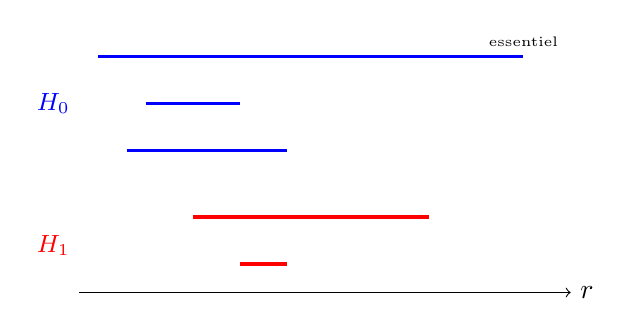
\begin{tikzpicture}[scale=1.2]
  \draw[->] (-0.2,0) -- (5,0) node[right] {$r$};
  % H_0 bars
  \draw[blue, very thick] (0, 2.5) -- (4.5, 2.5);
  \draw[blue, very thick] (0.5, 2.0) -- (1.5, 2.0);
  \draw[blue, very thick] (0.3, 1.5) -- (2.0, 1.5);
  % H_1 bars
  \draw[red, very thick] (1.0, 0.8) -- (3.5, 0.8);
  \draw[red, very thick] (1.5, 0.3) -- (2.0, 0.3);
  % Labels
  \node[left, font=\small, blue] at (-0.2, 2.0) {$H_0$};
  \node[left, font=\small, red] at (-0.2, 0.5) {$H_1$};
  \node[above, font=\tiny] at (4.5, 2.5) {essentiel};
\end{tikzpicture}
\end{center}

\begin{remarque}
Le code-barres et le diagramme de persistance contiennent exactement la
m\^eme information. Le code-barres est souvent plus intuitif pour la
visualisation~; le diagramme est plus adapt\'e \`a l'analyse
math\'ematique (distances, stabilit\'e).
\end{remarque}

% ============================================================
\section{Fonctions de Betti}
% ============================================================

\begin{definition}[Fonction de Betti]
La \emph{fonction de Betti} $\beta_p : \R \to \N$ associe \`a chaque
$r \in \R$ le nombre de Betti du complexe filtr\'e au niveau $r$~:
\[
  \beta_p(r) = \dim H_p(K_r).
\]
C'est une fonction en escalier, croissante par morceaux.
\end{definition}

\begin{proposition}
La fonction de Betti $\beta_p(r)$ peut se lire directement du
code-barres~: $\beta_p(r)$ est le nombre de barres qui contiennent $r$
en dimension $p$.
\end{proposition}

% ============================================================
\section{Paysages de persistance}
% ============================================================

\begin{definition}[Paysage de persistance]
Soit $\mathrm{Dgm}_p = \{(b_i, d_i)\}$. Pour chaque point, d\'efinir
la fonction tente~:
\[
  \Lambda_i(t) = \max\left(0,\, \min(t - b_i,\, d_i - t)\right).
\]
Le \emph{$k$-i\`eme paysage de persistance} est~:
\[
  \lambda_k(t) = k\text{-i\`eme plus grande valeur de }
  \{\Lambda_i(t)\}_{i=1}^N.
\]
\end{definition}

\begin{formules}[title=\textbf{Paysage de persistance}]
\[
  \lambda_k : \R \to \R_{\geq 0}, \quad
  \lambda_k(t) = \mathrm{kmax}\big\{\Lambda_i(t) : (b_i, d_i)
  \in \mathrm{Dgm}_p\big\}
\]
o\`u $\mathrm{kmax}$ d\'enote le $k$-i\`eme maximum.
\end{formules}

\begin{theoreme}[Bubenik, 2015]
Les paysages de persistance sont des \'el\'ements d'un espace de Banach
s\'eparable. Ils v\'erifient une loi forte des grands nombres et un
th\'eor\`eme central limite.
\end{theoreme}

% ============================================================
\section{Images de persistance}
% ============================================================

\begin{definition}[Image de persistance]
L'\emph{image de persistance} (\emph{persistence image}) est obtenue
en~:
\begin{enumerate}
  \item Transformant chaque point $(b, d)$ en $(b, d-b)$ (coordonn\'ees
        naissance-persistance).
  \item Pla\c{c}ant une gaussienne $\mathcal{N}((b_i, p_i), \sigma^2 I)$
        centr\'ee sur chaque point transform\'e.
  \item Pond\'erant par une fonction de poids $w(b, p)$ (typiquement
        croissante en $p$).
  \item Discr\'etisant sur une grille pour obtenir une matrice.
\end{enumerate}
\end{definition}

\begin{formules}[title=\textbf{Image de persistance}]
\[
  \rho(x, y) = \sum_{i=1}^{N} w(b_i, p_i) \cdot
  \frac{1}{2\pi\sigma^2}
  \exp\left(-\frac{(x - b_i)^2 + (y - p_i)^2}{2\sigma^2}\right)
\]
o\`u $p_i = d_i - b_i$ est la persistance du $i$-\`eme point.
\end{formules}

% ============================================================
\section{Impl\'ementation des repr\'esentations}
% ============================================================

\begin{codeblock}[title=\textbf{Visualisation des diagrammes et codes-barres}]
\begin{minted}{python}
import numpy as np
from ripser import ripser
from persim import plot_diagrams
import matplotlib.pyplot as plt

# Cercle bruité
theta = np.linspace(0, 2*np.pi, 100, endpoint=False)
X = np.column_stack([np.cos(theta), np.sin(theta)])
X += 0.1 * np.random.randn(*X.shape)

result = ripser(X, maxdim=1)
dgms = result['dgms']

fig, axes = plt.subplots(1, 3, figsize=(15, 4))

# Diagramme de persistance
plot_diagrams(dgms, ax=axes[0])
axes[0].set_title("Diagramme de persistance")

# Code-barres
for dim, dgm in enumerate(dgms):
    color = ['blue', 'red'][dim]
    offset = 0 if dim == 0 else len(dgms[0])
    for k, (b, d) in enumerate(dgm):
        if np.isinf(d):
            d = max(dgm[np.isfinite(dgm[:, 1]), 1].max(), b + 0.5)
        axes[1].plot([b, d], [k + offset, k + offset],
                     color=color, linewidth=2)
axes[1].set_title("Code-barres")
axes[1].set_xlabel("$r$")

# Paysage de persistance
t = np.linspace(0, 2.5, 500)
dgm1 = dgms[1]
dgm1_finite = dgm1[np.isfinite(dgm1[:, 1])]
tents = np.array([np.maximum(0, np.minimum(t - b, d - t))
                   for b, d in dgm1_finite])
if len(tents) > 0:
    landscape_1 = np.sort(tents, axis=0)[::-1]
    for k in range(min(3, len(landscape_1))):
        axes[2].plot(t, landscape_1[k], label=f"$\\lambda_{k+1}$")
    axes[2].legend()
axes[2].set_title("Paysages de persistance ($H_1$)")

plt.tight_layout()
plt.savefig("representations_persistance.pdf")
\end{minted}
\end{codeblock}

\begin{codeblock}[title=\textbf{Images de persistance avec giotto-tda}]
\begin{minted}{python}
from gtda.homology import VietorisRipsPersistence
from gtda.diagrams import PersistenceImage
import numpy as np

# Données
theta = np.linspace(0, 2*np.pi, 100, endpoint=False)
X = np.column_stack([np.cos(theta), np.sin(theta)])
X += 0.1 * np.random.randn(*X.shape)

# Pipeline giotto-tda
VR = VietorisRipsPersistence(homology_dimensions=[0, 1])
diagrams = VR.fit_transform(X[np.newaxis, :, :])

PI = PersistenceImage(sigma=0.1, n_bins=20)
images = PI.fit_transform(diagrams)
print(f"Forme de l'image de persistance: {images.shape}")
\end{minted}
\end{codeblock}

% ============================================================
\section{Entropie de persistance}
% ============================================================

\begin{definition}[Entropie de persistance]
Soit $\mathrm{Dgm} = \{(b_i, d_i)\}_{i=1}^N$ un diagramme de
persistance (points finis seulement). L'\emph{entropie de persistance}
est~:
\[
  E(\mathrm{Dgm}) = -\sum_{i=1}^{N} p_i \log p_i, \quad
  p_i = \frac{d_i - b_i}{\sum_{j=1}^N (d_j - b_j)}.
\]
Elle mesure la complexit\'e de la distribution des persistances.
\end{definition}

% ============================================================
\section{Courbe de Betti}
% ============================================================

\begin{definition}[Courbe de Betti]
La \emph{courbe de Betti} est la fonction $\beta_p : \R \to \N$
d\'efinie par~:
\[
  \beta_p(t) = \abs{\{(b_i, d_i) \in \mathrm{Dgm}_p : b_i \leq t < d_i\}}.
\]
\end{definition}

Cette courbe est directement li\'ee au code-barres~: elle compte le
nombre de barres actives \`a chaque instant $t$.

% ============================================================
\section{Silhouettes de persistance}
% ============================================================

\begin{definition}[Silhouette de persistance]
La \emph{silhouette de persistance} d'ordre $q > 0$ est la moyenne
pond\'er\'ee des fonctions tentes~:
\[
  \phi_q(t) = \frac{\sum_i (d_i - b_i)^q \cdot \Lambda_i(t)}
  {\sum_i (d_i - b_i)^q}.
\]
Pour $q = 1$, c'est la moyenne arithm\'etique pond\'er\'ee par la
persistance.
\end{definition}

% ============================================================
\section{Statistiques sur les diagrammes}
% ============================================================

\begin{theoreme}[Moyenne de Fr\'echet]
Soit $\mathcal{D} = \{D_1, \ldots, D_n\}$ un \'echantillon de
diagrammes de persistance. La \emph{moyenne de Fr\'echet} est~:
\[
  \bar{D} = \arg\min_{D} \sum_{i=1}^n W_2(D, D_i)^2
\]
o\`u $W_2$ est la distance de Wasserstein d'ordre~$2$. Ce minimum
existe mais n'est pas n\'ecessairement unique.
\end{theoreme}

\begin{proposition}
Les paysages de persistance, \'etant des \'el\'ements d'un espace de
Banach, admettent une moyenne bien d\'efinie~:
\[
  \bar{\lambda}_k(t) = \frac{1}{n} \sum_{i=1}^n \lambda_k^{(i)}(t).
\]
\end{proposition}

% ============================================================
\section{Exercices}
% ============================================================

\begin{exercice}
Construire le diagramme de persistance et le code-barres pour une
filtration de Vietoris--Rips de $6$ points r\'eguli\`erement espac\'es
sur un cercle.
\end{exercice}

\begin{exercice}
Impl\'ementer en Python le calcul d'un paysage de persistance \`a
partir d'un diagramme de persistance. Tester sur un cercle bruit\'e.
\end{exercice}

\begin{exercice}
Calculer l'image de persistance d'un nuage de $200$ points sur un tore.
Faire varier le param\`etre $\sigma$ et observer l'effet sur l'image.
\end{exercice}

\begin{exercice}
Montrer que l'entropie de persistance est maximale lorsque toutes les
persistances sont \'egales, et minimale (nulle) lorsqu'une seule paire
a une persistance non nulle.
\end{exercice}

\begin{exercice}
Comparer les paysages de persistance d'un cercle, d'un tore et d'une
sph\`ere \'echantillonn\'es avec du bruit. Quelles diff\'erences
observe-t-on~?
\end{exercice}
